\documentclass[a3paper,12pt]{extarticle} % Use extarticle for A3 paper size
\usepackage{graphicx} % Include this package for \includegraphics
\usepackage{amsmath}
\usepackage{amssymb} % Include this package for \mathbb
\usepackage[margin=1in]{geometry} % Adjust the margin as needed

\begin{document}

\author{kipngeno koech - bkoech}
\title{Homework 1 - Introduction to Probabilistic Graphical Models}   
\maketitle

\medskip

\maketitle

\section{Bayesian Networks}

\begin{enumerate}
\item Consider a simple Markov Chain structure \( X \rightarrow Y \rightarrow Z \), where all variables are binary. You are required to:
\begin{enumerate}
    \item Write a code (using your preferred programming language) that generates a distribution (not necessarily a valid BN one) over the 3 variables.
        \[\textbf{[ in the notebook]}\]
    \item Write a code that verifies whether a distribution is a valid BN distribution.
        \[\textbf{[ in the notebook ]}\]
    \item Using your code, generate 10000 distributions and compute the fraction of distributions that are valid BN distributions.
        \[\textbf{ [ in the notebook ]}\]
\end{enumerate}
\item Given the following Bayesian Network
\begin{figure}[h]
    \centering
    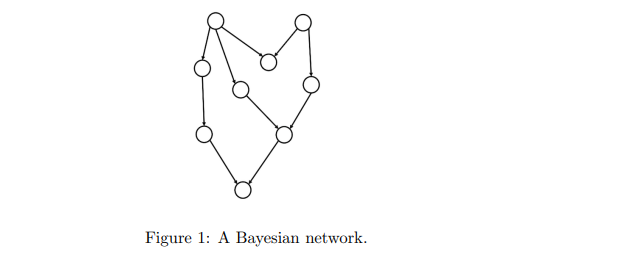
\includegraphics[width=0.5\textwidth]{bn.png}
    \caption{Bayesian Network}
\end{figure}
\begin{enumerate}
    \item Propose a topological ordering of this graph
    \begin{figure}[h]
        \centering
        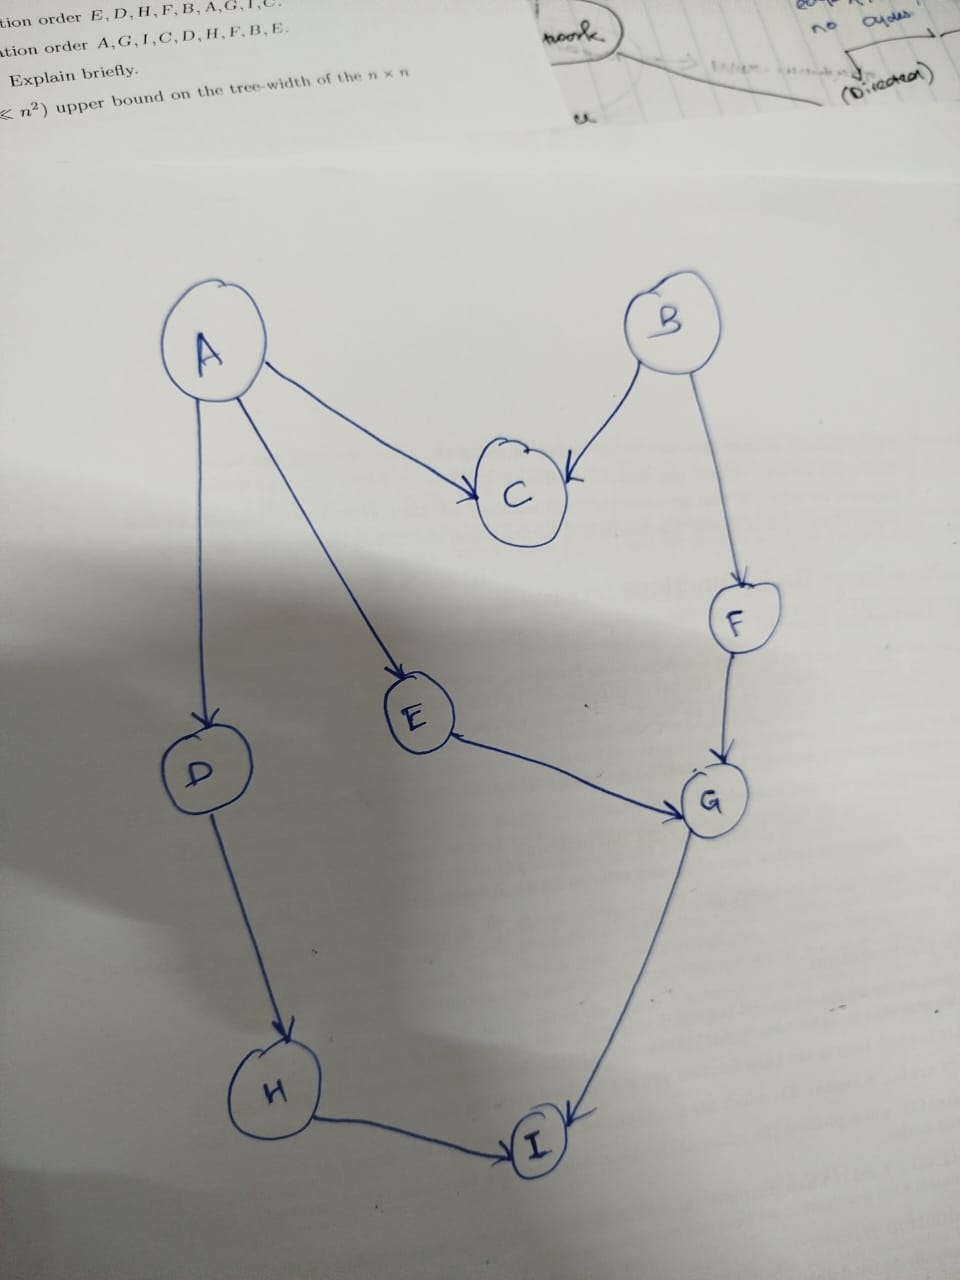
\includegraphics[width=0.5\textwidth]{bn1.jpg}
        \caption{Bayesian Network}
    \end{figure}
    \\ In Figure 2, the topological ordering is:
    \begin{enumerate}
        \item \(A \rightarrow B \rightarrow C \rightarrow D \rightarrow E \rightarrow F \rightarrow G \rightarrow H \rightarrow I \)
        \item \(A \rightarrow B \rightarrow C \rightarrow E \rightarrow D \rightarrow F \rightarrow G \rightarrow I \rightarrow H \)
    \end{enumerate}
    \item Let \(\textbf{X}\) be a random vector that is Markov with respect to the graph. We assume that the random variables X, are binary. Write all the local conditional independence
    \[
        X_A \text{ has no parents, so no independence condition applies here.} 
    \]
    \[
        X_B \text{ has no parents, so no independence condition applies here.} \\
    \]
    \(X_C \text{ is conditionally independent of all other nodes given its parent } X_A: \)
    \[
        X_C \perp \{X_B, X_D, X_E, X_F, X_G, X_H, X_I\} \mid X_A \\
    \]
    \(
        X_D \text{ is conditionally independent of all other nodes given its parent } X_A: \\
    \)
    \[
        X_D \perp \{X_B, X_C, X_E, X_F, X_G, X_H, X_I\} \mid X_A \\
    \]
    \(
        X_E \text{ is conditionally independent of all other nodes given its parents } X_C \text{ and } X_D: \\
    \)
    \[
        X_E \perp \{X_A, X_B, X_F, X_G, X_H, X_I\} \mid \{X_C, X_D\} \\
    \]
    \(
        X_F \text{ is conditionally independent of all other nodes given its parent } X_B: \\
    \)
    \[
        X_F \perp \{X_A, X_C, X_D, X_E, X_G, X_H, X_I\} \mid X_B \\
    \]
    \(
        X_G \text{ is conditionally independent of all other nodes given its parents } X_E \text{ and } X_F: \\
    \)
    \[
        X_G \perp \{X_A, X_B, X_C, X_D, X_H, X_I\} \mid \{X_E, X_F\} \\
    \]
    \(
        X_H \text{ is conditionally independent of all other nodes given its parent } X_D: \\
    \)
    \[
        X_H \perp \{X_A, X_B, X_C, X_E, X_F, X_G, X_I\} \mid X_D \\
    \]
    \(
        X_I \text{ is conditionally independent of all other nodes given its parents } X_G \text{ and } X_H: \\
    \)
    \[
        X_I \perp \{X_A, X_B, X_C, X_D, X_E, X_F\} \mid \{X_G, X_H\}
    \]
\end{enumerate}
\item  State True or False, and briefly justify your answer within 3 lines. The statements are either
direct consequences of theorems in Koller and Friedman (2009, Ch. 3), or have a short proof. In the
follows, P is a distribution and G is a BN structure.
\begin{enumerate}
    \item If \( A \perp B \mid C \) and \( A \perp C \mid B \), then \( A \perp B \) and \( A \perp C \). (Suppose the joint distribution of \( A, B, C \) is positive.) (This is a general probability question not related to BNs.)
    \begin{itemize}
        \item \textbf{False}. Conditional independence does not imply marginal independence. For example, \( A \) and \( B \) can be dependent but become independent given \( C \).
    \end{itemize}
    \begin{figure}[h]
        \centering
        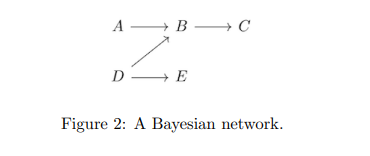
\includegraphics[width=0.5\textwidth]{bn2.png}
        \caption{Bayesian Network}
    \end{figure}
    \item In Figure 2, \(E \perp C \mid B\)
    \item in Figure 2, \(A \perp E \mid C\)
    \begin{figure}[h]
        \centering
        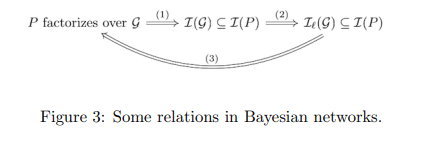
\includegraphics[width=0.5\textwidth]{bn3.png}
    \end{figure}
    \\\\ In figure 3, 
Recall the definitions of local and global independences of \( G \) and independences of \( P \).
\[
I_l(G) = \{(X \perp \text{NonDescendants}_G(X) \mid \text{Parents}_G(X))\} \tag{1}
\]
\[
I(G) = \{(X \perp Y \mid Z) : \text{d-separated}_G(X, Y \mid Z)\} \tag{2}
\]
\[
I(P) = \{(X \perp Y \mid Z) : P(X, Y \mid Z) = P(X \mid Z)P(Y \mid Z)\} \tag{3}
\]
\item In Figure 3, relation 1 is true.
\item In Figure 3, relation 2 is true.
\item In Figure 3, relation 3 is true.
\item If \( G \) is an I-map for \( P \), then \( P \) may have extra conditional independencies than \( G \).
\item Two BN structures \( G_1 \) and \( G_2 \) are I-equivalent if they have the same skeleton and the same set of v-structures.
\item If \( G_1 \) is an I-map of distribution \( P \), and \( G_1 \) has fewer edges than \( G_2 \), then \( G_2 \) is not a minimal I-map of \( P \).
\item The P-map of a distribution, if it exists, is unique.
\end{enumerate}
\end{enumerate}



\end{document}